\documentclass{article}

\usepackage{graphicx}
\usepackage{tikz}
\usepackage{tikzsymbols}
\usetikzlibrary{calc,patterns,shapes.geometric}
\pagestyle{empty}
\usepackage[margin=0pt]{geometry}
\geometry{papersize={14in,12in}}

\def\centerarc[#1](#2)(#3:#4:#5){\draw[#1] ($(#2)+({#5*cos(#3)},{#5*sin(#3)})$) arc (#3:#4:#5);}

\begin{document}
	\begin{figure}
		\centering
		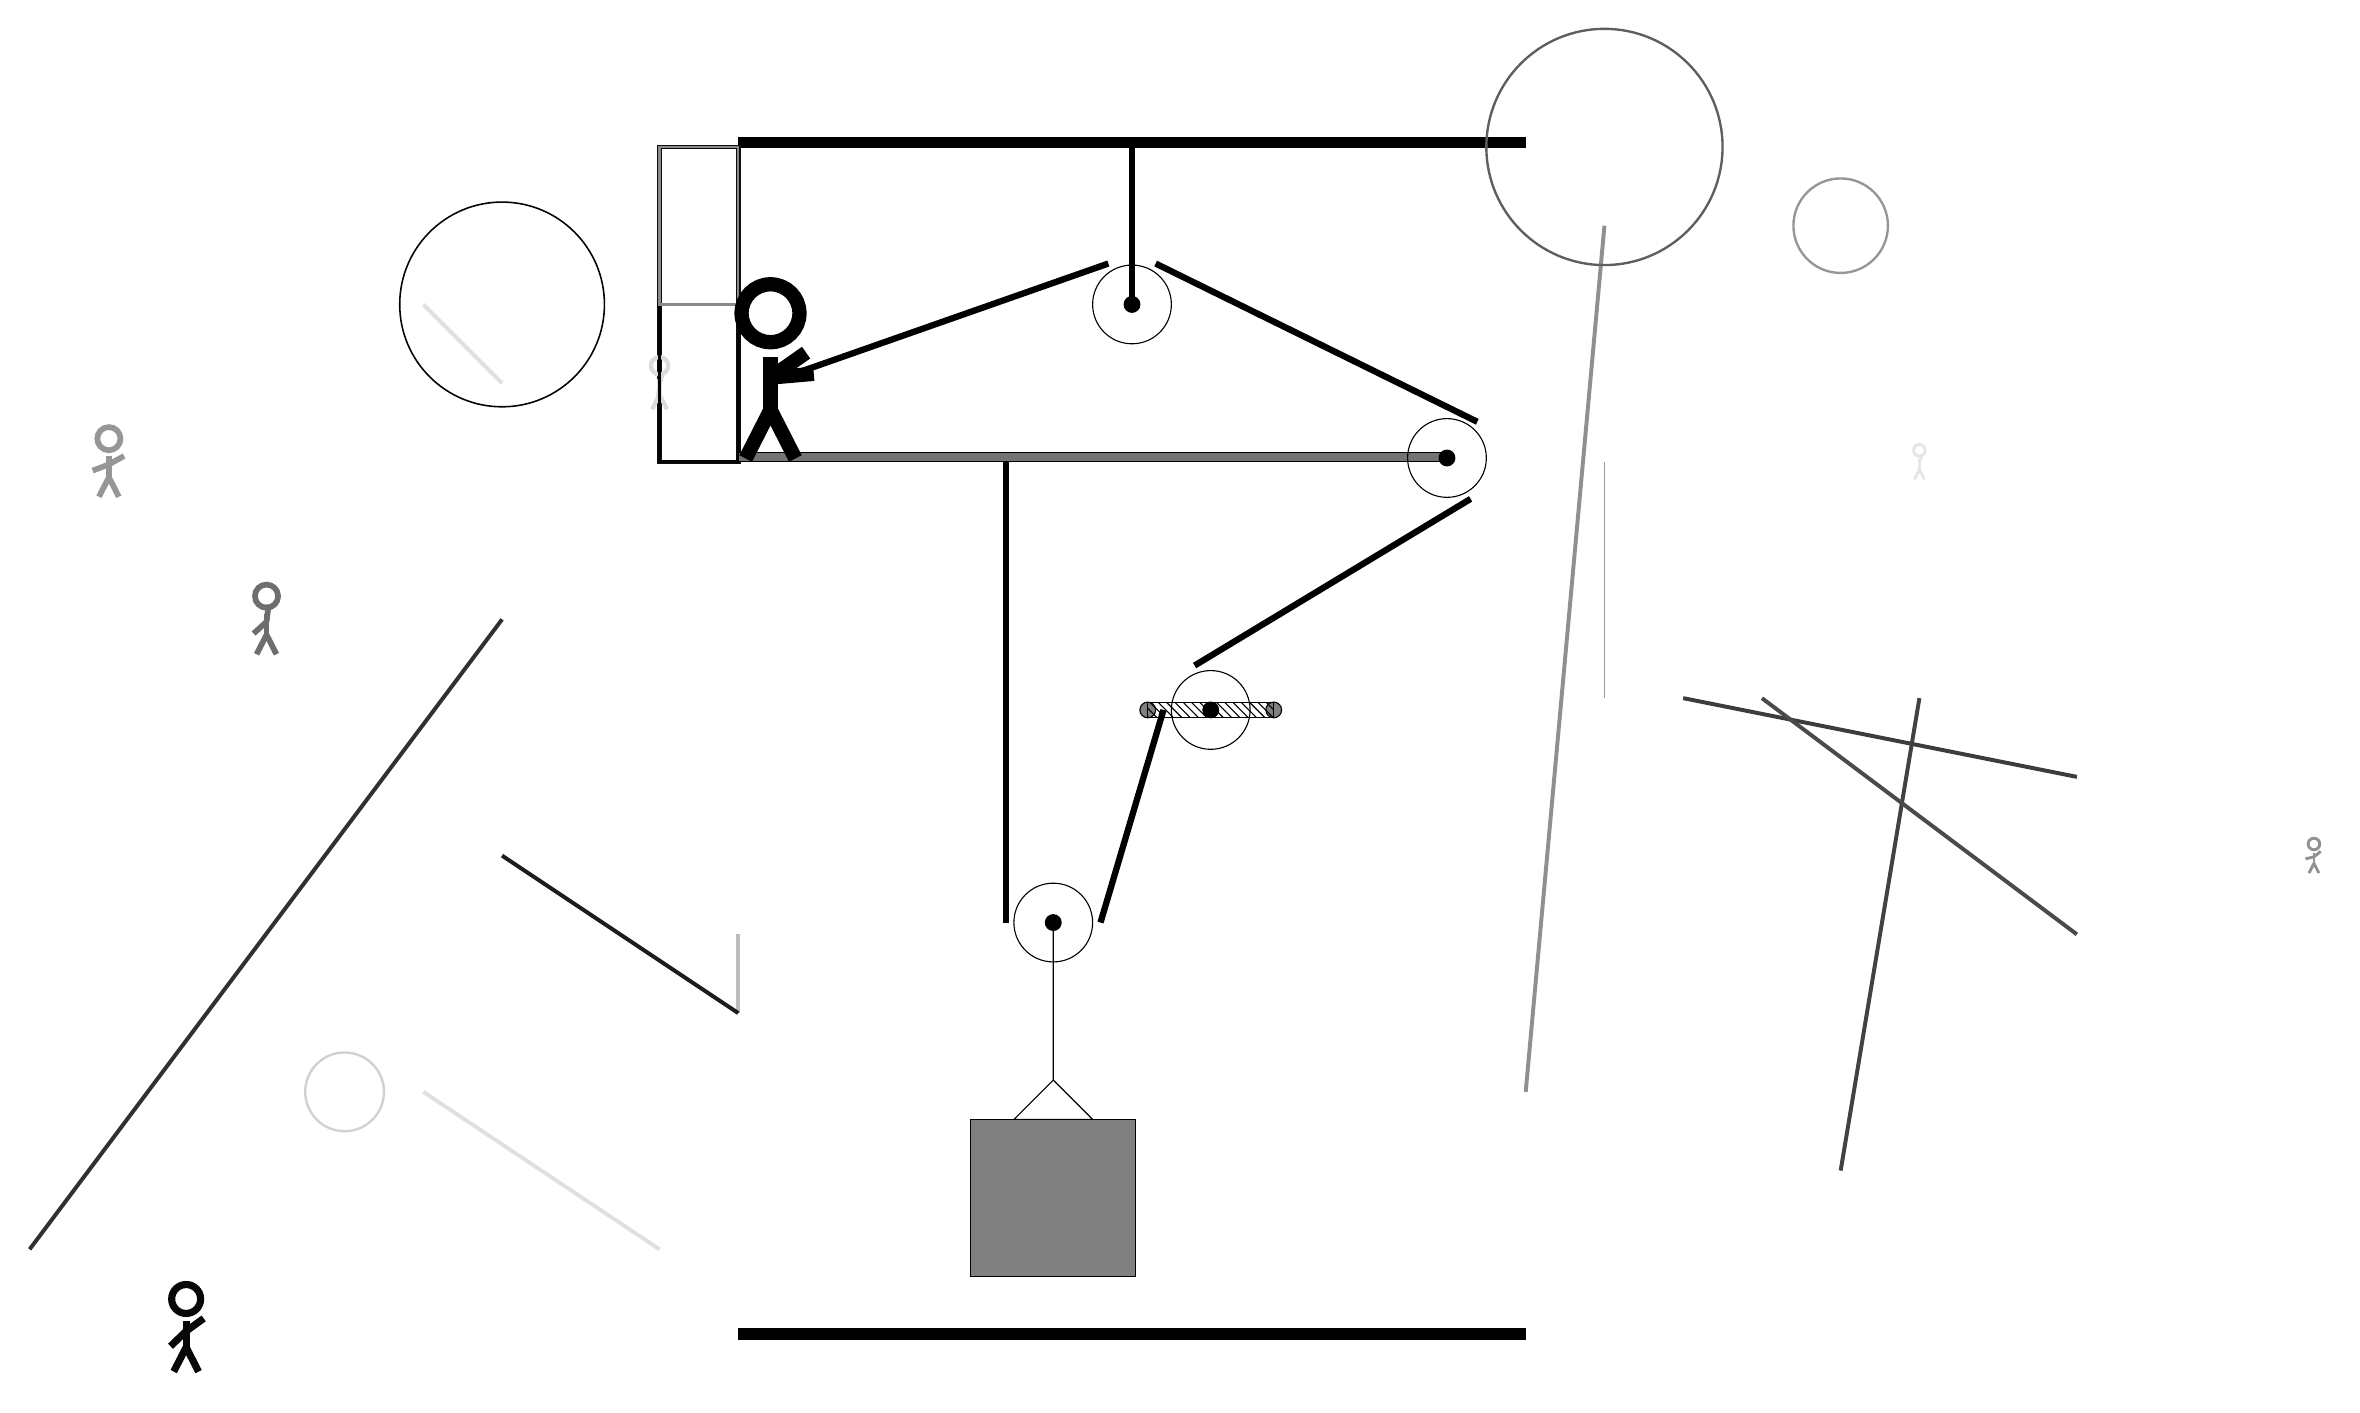
\begin{tikzpicture}
			%%%%% START %%%%%
			
			\draw[fill=black] (-2, 13) rectangle (8, 13.125);
			
			\draw[line width=0.5mm, color=black!12](-6, 1) -- (-3, -1);
			
			\draw[line width=0.5mm, color=black!44](9, 12) -- (8, 1);
			\draw[line width=0.5mm, color=black!74](13, 6) -- (12, 0);
			\draw[line width=0.5mm, color=black!12](-6, 11) -- (-5, 10);
			
			\draw[line width=0.6mm, color=black!95] (-3, 9) rectangle (-2, 13);
			\draw[line width=0.5mm, color=black!26](-2, 2) -- (-2, 3);
			
			\node[line width=0.2mm, color=black!97] at (-9, -2) {\Strichmaxerl[5][44][36]};
			\draw[line width=0.5mm, color=black!76](10, 6) -- (15, 5);
			\draw [line width=0.3mm, color=black!63](9, 13) circle (1.5);
			\node[line width=0.5mm, color=black!14] at (-3, 10) {\Strichmaxerl[3][82][76]};
			
			\draw[line width=0.4mm, color=black!98] (-3, 11) rectangle (-2, 9);
			
			\node[line width=0.4mm, color=black!43] at (18, 4) {\Strichmaxerl[2][13][39]};
			\draw [line width=0.3mm, color=black!18](-7, 1) circle (0.5);
			
			\draw[line width=0.5mm, color=black!89](-5, 4) -- (-2, 2);
			\draw[line width=0.3mm, color=black!46] (-3, 13) rectangle (-2, 11);
			\draw[line width=0.5mm, color=black!71](11, 6) -- (15, 3);
			
			\draw[line width=0.2mm, color=black!40] (9, 9) rectangle (9, 6);
			\draw [line width=0.2mm, color=black!99](-5, 11) circle (1.3);
			\draw[line width=0.5mm, color=black!81](-5, 7) -- (-11, -1);
			
			\draw [line width=0.3mm, color=black!41](12, 12) circle (0.6);
			\node[line width=0.4mm, color=black!10] at (13, 9) {\Strichmaxerl[2][90][76]};
			
			\node[line width=0.5mm, color=black!41] at (-10, 9) {\Strichmaxerl[4][21][29]};
			\node[line width=0.5mm, color=black!57] at (-8, 7) {\Strichmaxerl[4][42][83]};
			
			\draw[fill=black!55] (-2, 9) rectangle (7, 9.125);
			
			\draw (2, 3.15) circle (0.5);
			\draw[fill=black] (2, 3.15) circle (0.1);
			
			\draw (7, 9.05) circle (0.5);
			\draw[fill=black] (7, 9.05) circle (0.1);
			
			\draw[fill=white](4, 5.85) circle (0.5);
			\draw[fill=black] (4, 5.85) circle (0.1);
			\draw[fill=black!50] (3.2, 5.85) circle (0.1);
			\draw[fill=black!50] (4.8, 5.85) circle (0.1);
			\draw[pattern=north west lines, pattern color=black] (3.2, 5.95) rectangle (4.8, 5.75);
			
			\draw (3, 11) circle (0.5);
			\draw[fill=black] (3, 11) circle (0.1);
			\draw[line width=0.8mm] (3, 11) -- (3, 13);
			
			\draw (2, 3.15) -- (2, 1.15) -- (1.5, 0.65) -- (2.5, 0.65) -- (2, 1.15);
			\draw[fill=black!50] (0.95, 0.65) rectangle (3.05, -1.35);
			
			\draw[line width=0.8mm] (1.4, 9) -- (1.4, 3.15);
			\centerarc[line width=0.8mm](2, 3.15)(180:360:0.6);
			\draw[line width=0.8mm](2.6, 3.15) -- (3.4, 5.85);
			\centerarc[line width=0.8mm](4, 5.85)(110:180:0.6);
			\draw[line width=0.8mm](3.7948, 6.4138) -- (7.3, 8.5304);
			\centerarc[line width=0.8mm](7, 9.05)(-60:50:0.6);
			\draw[line width=0.8mm](7.3857, 9.5096) -- (3.3, 11.5196);
			\centerarc[line width=0.8mm](3, 11)(60:120:0.6);
			\draw[line width=0.8mm](2.7, 11.5196) -- (-1.2, 10.15);
			
			\node at (-1.5, 10.15) {\Strichmaxerl[10][-175][35]};
			
			\draw[fill=black] (-2, -2) rectangle (8, -2.15);
			
			%%%%% END %%%%%
		\end{tikzpicture}
	\end{figure}	
\end{document}